\chapter{Evolución de la enfermedad en un entorno controlado}

A continuación nos situaremos en un escenario un poco más realista. Supongamos que se descubre el inicio de un brote de gripa en el hospital de un pueblo con 49 personas y deseamos analizar el comportamiento de la enfermedad para establecer medidas de control para variaciones futuras de la misma gripa.

En el pueblo podemos identificar cinco lugares diferentes en donde las células interactúan entre sí: La escuela, las oficinas, el mercado, el hospital y las viviendas de cada persona. Asumiremos que en la población se realizó un censo y tenemos acceso a las edades de cada individuo, su lugar de trabajo (o donde pasan la mayor parte del tiempo) y las personas con las que viven. Distribuyéndose de la siguiente manera:

\begin{itemize}
    \item \textbf{Escuela (E):} Se sabe que en el pueblo hay 9 niños y 2 profesores.
    \item \textbf{Oficinas (O):} Cuenta con un personal de 16 individuos.
    \item \textbf{Mercado (M):} Se identificaron 8 trabajadores.
    \item \textbf{Hospital (H):} Entre doctores, enfermeros y pacientes se identifica una cantidad de 14 individuos.
\end{itemize}

Supondremos que todos los niños del pueblo son hijos únicos y que las viviendas con tres individuos cuentan con al menos un niño. Además de esto y de acuerdo con la información anterior supondremos que en el pueblo la población vive en uno de tres tipos de vivienda: la vivienda C1 en donde vive una sola persona y que se asume además que es un adulto; las viviendas C2 en donde viven dos individuos, ya sean dos adultos o un adulto y un niño; y por último las viviendas C3, en donde viven 3 personas.

\begin{figure}[h]\label{fig:edadesYOcupaciones}
  \centering
    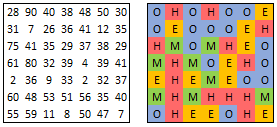
\includegraphics[width=0.3525\textwidth]{Imagenes/edadesYOcupaciones.PNG}
    \caption{Edades y ocupaciones en el pueblo.}
\end{figure}

De acuerdo con lo mencionado en el capítulo anterior, debemos establecer los grados de impacto de acuerdo con la manera en la que se distribuye nuestra población. En nuestro caso asumiremos que las personas que viven juntas tienen una grado de impacto cero entre ellas, que con los que tienen contacto en el lugar de ocupación tienen un grado de impacto igual a uno y que con las demás células tienen grado de impacto dos. De ese modo, si organizamos a la población sobre una malla identificando sus edades, ocupaciones y vecindades obtendremos algo como lo que se ve en la siguiente figura:

\begin{figure}[h]\label{fig:edadesYOcupaciones}
  \centering
    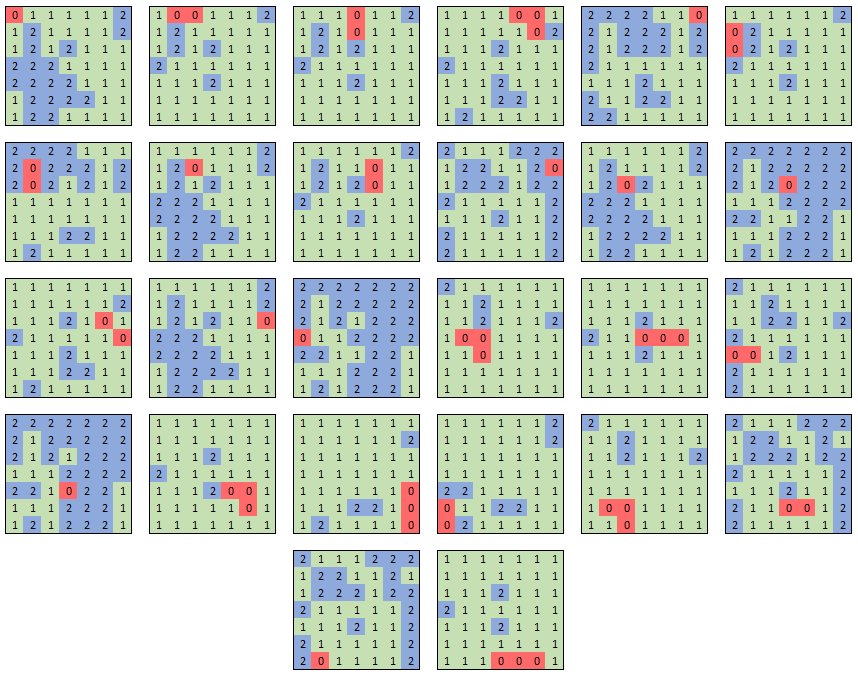
\includegraphics[width=1\textwidth]{Imagenes/vecindadesCap4.PNG}
    \caption{Grados de impacto.}
\end{figure}

En el caso de la enfermedad, supondremos que dura en promedio 5 días, por lo que tomaremos $\alpha=\frac{1}{5}=0.2$ y, por otro lado, tomaremos una tasa de infección $\beta=0.3$. Supondremos unas tasas de natalidad y de mortalidad iguales a 0.02 y 0.005 respectivamente y finalmente, asumiremos que de brotes de gripa anteriores se tiene que las tasas de letalidad de la enfermedad son:

%%%%%%%%%%%%%%%%%%%%%%%%%%%%%%%%%%%%%%%%%%%%%%%%%%%%%%%%%%%%%%%%%%%%%%%%%%%%%%%%%%%%%%%%%%%%%%
\newpage
%%%%%%%%%%%%%%%%%%%%%%%%%%%%%%%%%%%%%%%%%%%%%%%%%%%%%%%%%%%%%%%%%%%%%%%%%%%%%%%%%%%%%%%%%%%%%%

\begin{table}[h]
\begin{center}
\begin{tabular}{| c | c |}
\hline
Rango de edades & Tasas \\ \hline
1 - 15 & 0.005 \\
16 - 48 & 0.01 \\
49 - 55 & 0.1 \\
56+ & 0.25 \\\hline
\end{tabular}
\caption{Tasas estimadas de letalidad de la gripa en el pueblo}
\end{center}
\end{table}

Analizaremos el comportamiento de la enfermedad en un periodo de 30 días tomando diferentes tasas de impacto. Esto nos brindará una visión de las implicaciones que pueden llegar a tener las relaciones más cercanas con individuos fuera de la vecindad mínimal en el evento donde se propaga alguna enfermedad.

\begin{figure}[h]
  \centering
    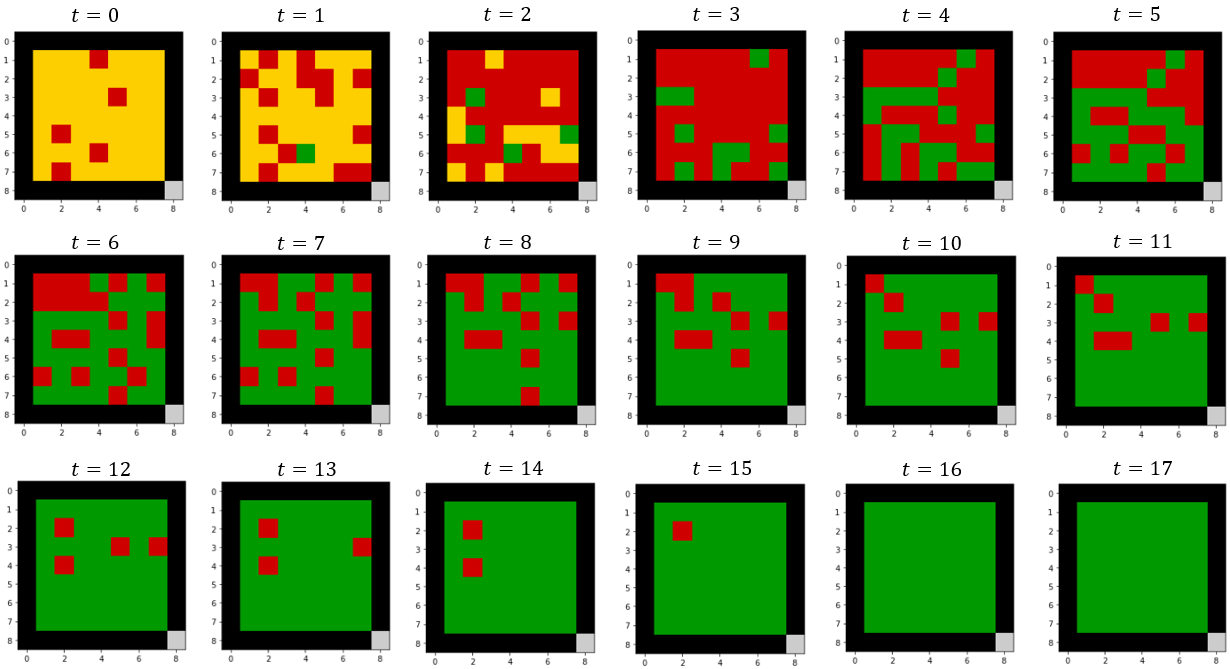
\includegraphics[width=1\textwidth]{Imagenes/evo1.PNG}
    \caption{Evolución de la enfermedad tomando como punto de inicio el hospital.}
    \label{fig:evo1}
\end{figure}

En el ejercicio de la figura \ref{fig:evo1} se puede observar que la enfermedad acaba desapareciendo en un periodo de 16 días, cabe resaltar que en algún momento toda la población contrajo la enfermedad y que la cantidad de casos empezó a disminuir desde el día 3. La figura \ref{fig:metricas1} nos muestra las cantidades de individuos por estado para un periodo de 30 días, mientras que en la tabla \ref{tab:tasasDeImpacto1} encontramos las tasas de impacto usadas durante el ejercicio.

%%%%%%%%%%%%%%%%%%%%%%%%%%%%%%%%%%%%%%%%%%%%%%%%%%%%%%%%%%%%%%%%%%%%%%%%%%%%%%%%%%%%%%%%%%%%%%
\newpage
%%%%%%%%%%%%%%%%%%%%%%%%%%%%%%%%%%%%%%%%%%%%%%%%%%%%%%%%%%%%%%%%%%%%%%%%%%%%%%%%%%%%%%%%%%%%%%

\begin{table}[h]
\begin{center}
\begin{tabular}{| c | c |}
\hline
Grados & Tasas \\ \hline
0 & 1 \\
1 & 0.5 \\
2 & 0.25 \\\hline
\end{tabular}
\caption{Tasas de impacto - Primer escenario}
\label{tab:tasasDeImpacto1}
\end{center}
\end{table}

\begin{figure}[h]
  \centering
    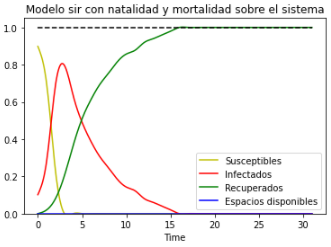
\includegraphics[width=0.5\textwidth]{Imagenes/metricas1.PNG}
    \caption{Cambios de estado con punto de inicio en el hospital. Escenario 1.}
    \label{fig:metricas1}
\end{figure}

Si ahora en lugar de esto suponemos que dentro del pueblo las relaciones son un poco más lejanas debido a periodos de alternancia, podemos asumir que las tasas de impacto son menores a las del ejercicio anterior. Para este escenario supondremos que las tasas de impacto son las descritas en la tabla \ref{tab:tasasDeImpacto2}.

\begin{table}[h]
\begin{center}
\begin{tabular}{| c | c |}
\hline
Grados & Tasas \\ \hline
0 & 1 \\
1 & 0.005 \\
2 & 0.0025 \\\hline
\end{tabular}
\caption{Tasas de impacto - Segundo escenario}
\label{tab:tasasDeImpacto2}
\end{center}
\end{table}

En la figura \ref{fig:metricas2} podemos apreciar que el pico que alcanza la enfermedad en el pueblo no es tan traumático en comparación con el alcanzado en el primer escenario, validando así la eficacia de medidas como los periodos de alternancia en las diferentes labores que se pueden ejercer dentro de la población.

%%%%%%%%%%%%%%%%%%%%%%%%%%%%%%%%%%%%%%%%%%%%%%%%%%%%%%%%%%%%%%%%%%%%%%%%%%%%%%%%%%%%%%%%%%%%%%
\newpage
%%%%%%%%%%%%%%%%%%%%%%%%%%%%%%%%%%%%%%%%%%%%%%%%%%%%%%%%%%%%%%%%%%%%%%%%%%%%%%%%%%%%%%%%%%%%%%

\begin{figure}[h]
  \centering
    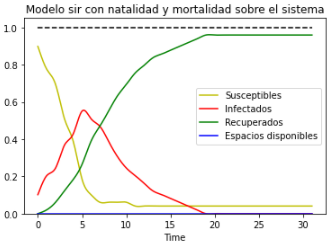
\includegraphics[width=0.5\textwidth]{Imagenes/metricas2.PNG}
    \caption{Cambios de estado con punto de inicio en el hospital. Escenario 2.}
    \label{fig:metricas2}
\end{figure}

Este escenario también nos permite ver que en el pueblo se alcanza lo que se conoce como inmunidad de rebaño dado que hay individuos que nunca se contagiaron de la enfermedad, lo cual se debe a la naturaleza de las interacciones consideradas. La figura \ref{fig:evo2} nos brinda un panorama más espacial de esta característica.

\begin{figure}[h]
  \centering
    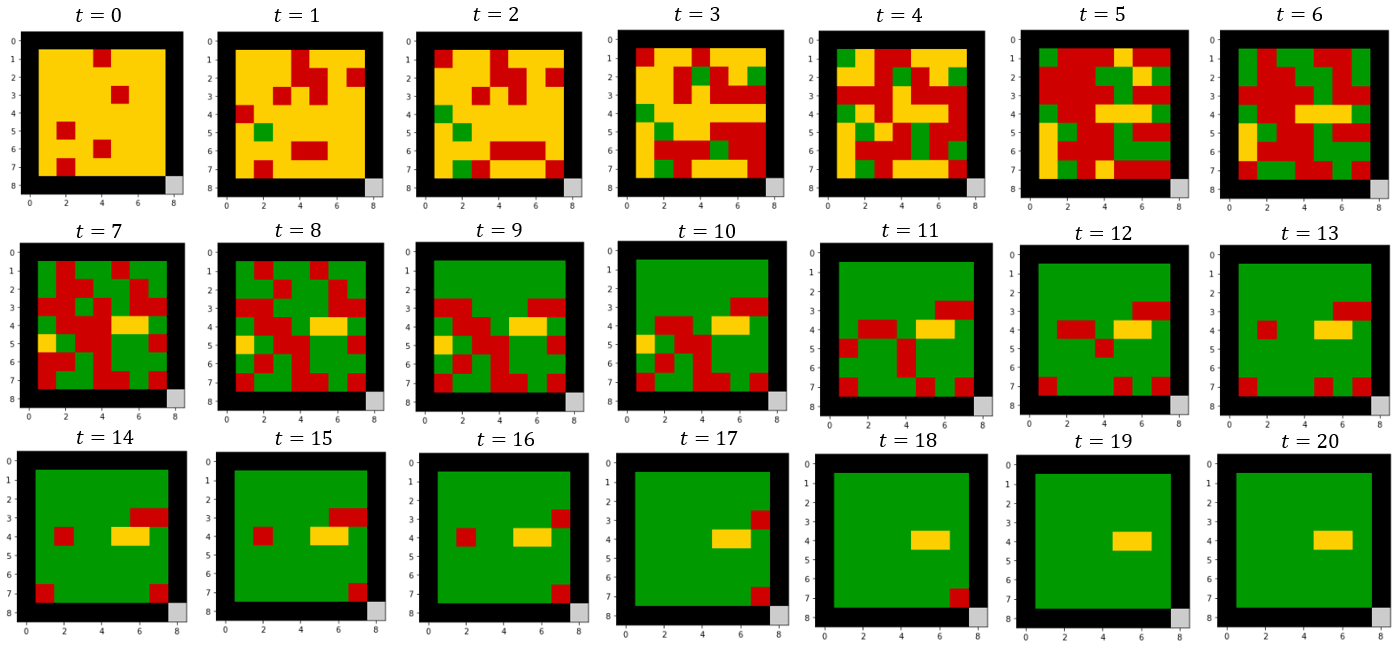
\includegraphics[width=1.05\textwidth]{Imagenes/evo2.PNG}
    \caption{Evolución de la enfermedad tomando como punto de inicio el hospital.}
    \label{fig:evo2}
\end{figure}

Cabe resaltar que a pesar de que la población está más distanciada, la enfermedad tiene un comportamiento similar a la del primer escenario. Esto se debe a la naturaleza descrita por los parámetros de la enfermedad y a su número básico de reproducción $\mathcal{R}_0$ (\ref{eq:R0}). En la figura \ref{fig:comparacionTasasdeImpacto} podremos observar la evolución promedio sobre 100 simulaciones de la enfermedad teniendo en cuenta diferentes tasas de impacto:

\begin{figure}[h]
  \centering
    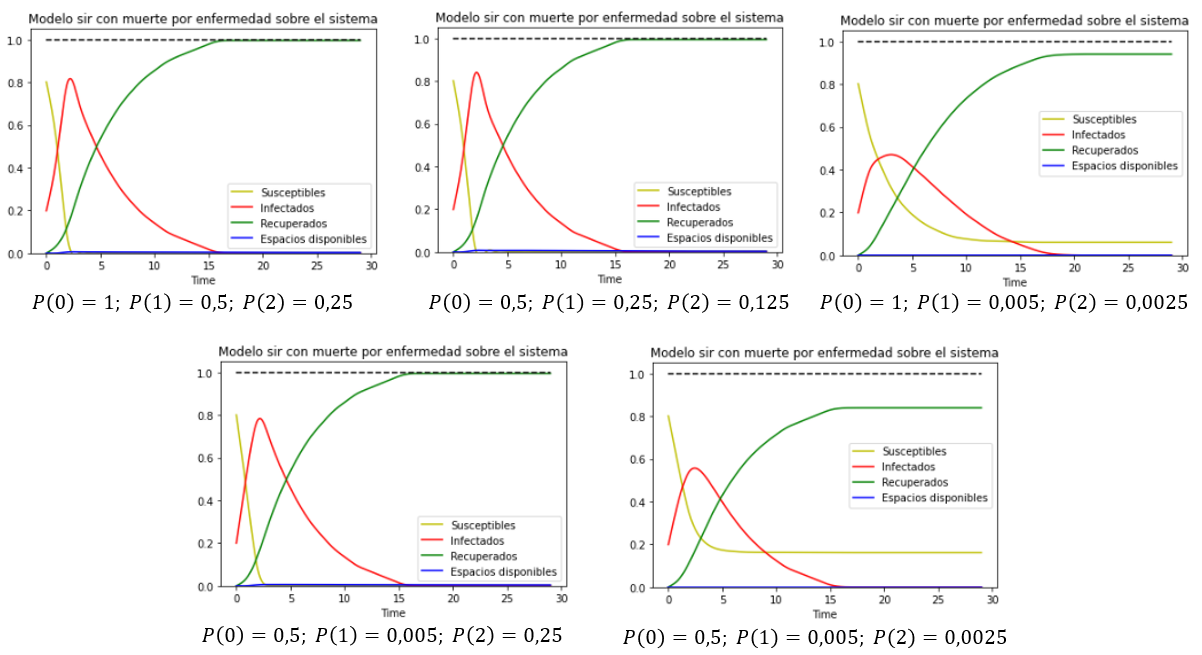
\includegraphics[width=1.05\textwidth]{Imagenes/comparacionTasasImpacto.PNG}
    \caption{Evolución promedio de la enfermedad tomando distintas tasas de impacto.}
    \label{fig:comparacionTasasdeImpacto}
\end{figure}

Durante todo el capítulo hemos estado trabajando al rededor de un escenario similar con un valor de $\mathcal{R}_0>1$ y en todos los ejercicios que abordamos, se puede evidenciar que la enfermedad alcanza un pico (o punto máximo de cantidad de contagios activos) en un momento similar. Esto se debe a que a pesar de considerar los mismos parámetros de la enfermedad, estamos modificando las propiedades en sí del espacio de células y esto a su vez, nos permite afirmar que la condición inicial no dependerá únicamente de los parámetros $\alpha$, $\beta$ y las tasas $\mu_k, \theta_k$ como ocurría en el modelo clásico, y en su lugar se tendrán que tomar en cuenta las maneras en las que las células pueden llegar a interactuar.

Afirmaciones como la anterior, nos motivan a preguntarnos si el sistema de vecindades con el que se describen las interacciones, tiene algún tipo de incidencia en el comportamiento de la enfermedad. Para responder a esta inquietud nos planteamos el escenario que se puede observar en la figura \ref{fig:comparacionTasasdeImpacto} en donde se muestra la evolución de la misma enfermedad, sobre un espacio en el que las relaciones entre células se pueden describir a partir de los sistemas de vecindades de Moore y de Von Neumann junto con el escenario planteado durante el presente capítulo. Para los tres escenarios se tomaron las curvas promedio para un total de 100 simulaciones.

%%%%%%%%%%%%%%%%%%%%%%%%%%%%%%%%%%%%%%%%%%%%%%%%%%%%%%%%%%%%%%%%%%%%%%%%%%%%%%%%%%%%%%%%%%%%%%
\newpage
%%%%%%%%%%%%%%%%%%%%%%%%%%%%%%%%%%%%%%%%%%%%%%%%%%%%%%%%%%%%%%%%%%%%%%%%%%%%%%%%%%%%%%%%%%%%%%

\begin{figure}[h]
  \centering
    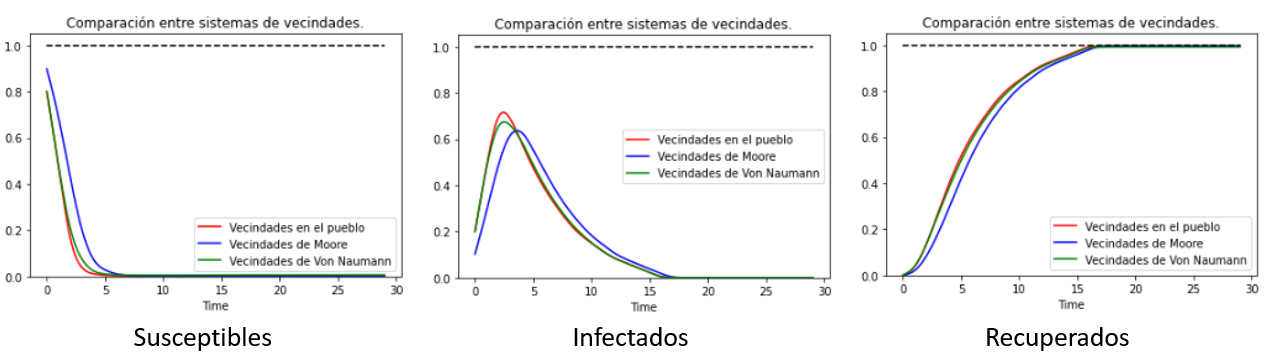
\includegraphics[width=1\textwidth]{Imagenes/comparacionSistemasVecindades.PNG}
    \caption{Evolución promedio de la enfermedad tomando tres sistemas de vecindades.}
    \label{fig:comparacionSistemasDeVecindades}
\end{figure}

La figura \ref{fig:comparacionSistemasDeVecindades} nos permite afirmar nuevamente que las condiciones espaciales y la manera en la que interactúan las células, si tiene un impacto en la manera en la que una enfermedad afecta a un conjunto de individuos y válida el hecho de que restringir las relaciones o la intensidad con la que pueden llegar a interactuar las células puede disminuir significativamente la cantidad de casos activos de la enfermedad como se vio en la figura \ref{fig:comparacionTasasdeImpacto}, generando así una mayor resiliencia por parte de las entidades que se encargan de la salud pública.